\documentclass[twoside,11pt]{homework}
\usepackage{color}
\usepackage{listings}
\usepackage{graphicx} 

\coursename{COMS W4733 Computational Aspects of Robotics} 

\studname{Jing Qian}    % YOUR NAME GOES HERE
\studmail{jq2282@columbia.edu}% YOUR UNI GOES HERE
\hwNo{2}                   % THE HOMEWORK NUMBER GOES HERE
\date{\today} % DATE GOES HERE


\begin{document}
\maketitle

\section*{Problem 1}

%%%%%%%%%%%%%%%%%%%%%%%%%%%%%%%%%%%%%%%%%%%%%%%%%%%%%
\section*{Problem 2}
(a)\\
\begin{equation}
\begin{split}
J_p(q) &= 
\begin{bmatrix}
\frac{\partial p_x}{\partial q_1} & \frac{\partial p_x}{\partial q_2} & \frac{\partial p_x}{\partial q_3} \\
\frac{\partial p_y}{\partial q_1} & \frac{\partial p_y}{\partial q_2} & \frac{\partial p_y}{\partial q_3}  \\
\frac{\partial p_z}{\partial q_1} & \frac{\partial p_z}{\partial q_2} & \frac{\partial p_z}{\partial q_3} 
\end{bmatrix}\\
&= \begin{bmatrix}
-(L_1+L_2c_2+L_3c_{23})s_1 & -L_2c_1s_2-L_3c_1s_{23} & -L_3c_1s_{23} \\
 (L_1+L_2c_2+L_3c_{23})c_1 & -L_2s_1s_2-L_3s_1s_{23} & -L_3s_1s_{23}  \\
0 & L_2c_2+L_3c_{23} & L_3c_{23}
\end{bmatrix}
\end{split}
\end{equation}

%
%%%%%%%%%%%%%%%%%%% Table. 1 %%%%%%%%%%%%%%%%%%%%%%%%%%%%%%
\begin{table}[h!] \centering
\caption{DH Parameter Table}
\begin{tabular}{|l|l|l|l|l|}
\hline
Link & $a_i$ & \textbf{$\alpha_i$} & $d_i$   & $\theta_i$ \\ \hline
1             & $L_1$            & 90                 & 0      & $\theta_1$ \\ \hline
2             & $L_2$           & 0                   &0      &  $\theta_2$       \\ \hline
3             & $L_3$             & 0                 & 0   & $\theta_3$        \\ \hline
\end{tabular}
\end{table}
%


%%%%%%%%%%%%%%%%%%%%%%%%%%%%%%%%%%%%%%%%%%%%%%%%%%%%%
\section*{Problem 3}
(a)\\
%
%%%%%%%%%%%%%%%%%%% Table. 1 %%%%%%%%%%%%%%%%%%%%%%%%%%%%%%
\begin{table}[h!] \centering
\caption{DH Parameter Table}
\begin{tabular}{|l|l|l|l|l|}
\hline
Link & $a_i$ & \textbf{$\alpha_i$} & $d_i$   & $\theta_i$ \\ \hline
1             & 1             & 90                 & 0      & $\theta_1$+90 \\ \hline
2             & 0             & -90                & $d_2$+2 & 0       \\ \hline
3             & 2             & 0                 & 0   & $\theta_3$-90        \\ \hline
\end{tabular}
\end{table}
%
\\\\
(c)\\
\begin{equation}
\begin{split}
A_1^0 &= R_z(\theta_1+90)R_x(-90) = \left[
\begin{matrix}
-\sin \theta_1 & -\cos \theta_1 & 0 & 0 \\
\cos \theta_1 & -\sin \theta_1 & 0 & 0 \\
0 & 0 & 1 & 0 \\
0 & 0 & 0 & 1
\end{matrix}
\right]
\begin{bmatrix}
1 & 0 & 0 & 0 \\
0 & 0 & 1 & 0 \\
0 & -1 & 0 & 0 \\
0 & 0 & 0 & 1 
\end{bmatrix}
\\
&= \left[
\begin{matrix}
-\sin \theta_1 & 0 & -\cos \theta_1 & 0  \\
\cos \theta_1 & 0 & -\sin \theta_1 & 0 \\
0 & -1 & 0 & 0 \\
0 & 0 & 0 & 1
\end{matrix}
\right]
\\
A_2^1 &= T_z(d_2)R_x(90) =
\begin{bmatrix}
1 & 0 & 0 & 0 \\
0 & 1 & 0& 0 \\
0 & 0 & 1 & d_2 \\
0 & 0 & 0 & 1 
\end{bmatrix}
\begin{bmatrix}
1 & 0 & 0 & 0 \\
0 & 0 & -1 & 0 \\
0 & 1 & 0 & 0 \\
0 & 0 & 0 & 1 
\end{bmatrix}
\\
&= \begin{bmatrix}
1 & 0 & 0 & 0 \\
0 & 0 & -1& 0 \\
0 & 1 & 0 &d_2\\
0 & 0 & 0 & 1 
\end{bmatrix}
\\
A_3^2 &= R_z(\theta_3-90)T_x(a_3) = 
\left[
\begin{matrix}
\sin \theta_3 & \cos \theta_3 & 0 & 0 \\
-\cos \theta_3 & \sin \theta_3 & 0 & 0 \\
0 & 0 & 1 & 0 \\
0 & 0 & 0 & 1
\end{matrix}
\right]
\begin{bmatrix}
1 & 0 & 0 & a_3 \\
0 & 1 & 0 & 0 \\
0 & 0 & 1 & 0 \\
0 & 0 & 0 & 1 
\end{bmatrix}
\\
&= \left[
\begin{matrix}
\sin \theta_3 & \cos \theta_3 & 0 & a_3\sin \theta_3 \\
-\cos \theta_3 & \sin \theta_3 & 0 & -a_3\cos \theta_3 \\
0 & 0 & 1 & 0 \\
0 & 0 & 0 & 1
\end{matrix}
\right]
\end{split}
\end{equation}
So we have:
\begin{equation}
T_n^0 = A_1^0 A_2^1 A_3^2 = \left[
\begin{matrix}
-\sin \theta_1 & 0 & -\cos \theta_1 & 0  \\
\cos \theta_1 & 0 & -\sin \theta_1 & 0 \\
0 & -1 & 0 & 0 \\
0 & 0 & 0 & 1
\end{matrix}
\right]
\begin{bmatrix}
1 & 0 & 0 & 0 \\
0 & 0 & -1& 0 \\
0 & 1 & 0 &d_2\\
0 & 0 & 0 & 1 
\end{bmatrix}
\left[
\begin{matrix}
\sin \theta_3 & \cos \theta_3 & 0 & a_3\sin \theta_3 \\
-\cos \theta_3 & \sin \theta_3 & 0 & -a_3\cos \theta_3 \\
0 & 0 & 1 & 0 \\
0 & 0 & 0 & 1
\end{matrix}
\right]
\end{equation}
\\\\
(d)
The workspace of the arm is like a donut, shown in Fig. 1. The inner  radius of the ring is 1 and the outer radius is 3.

%%%%%%%%%%%%%%%%%%%%%%%%%%%%%%%%%%%%%%%%%%%%%%%%%%%%%
\section*{Problem 3}
(a)\\
The coordinate frames on the manipulator is shown in Fig. 2.
%%
%%%%%%%%%%%%%%%%%%%% Fig. 2 %%%%%%%%%%%%%%%%%%%%%%%%%%%%%%
%\begin{figure}[h!]
%\centering
%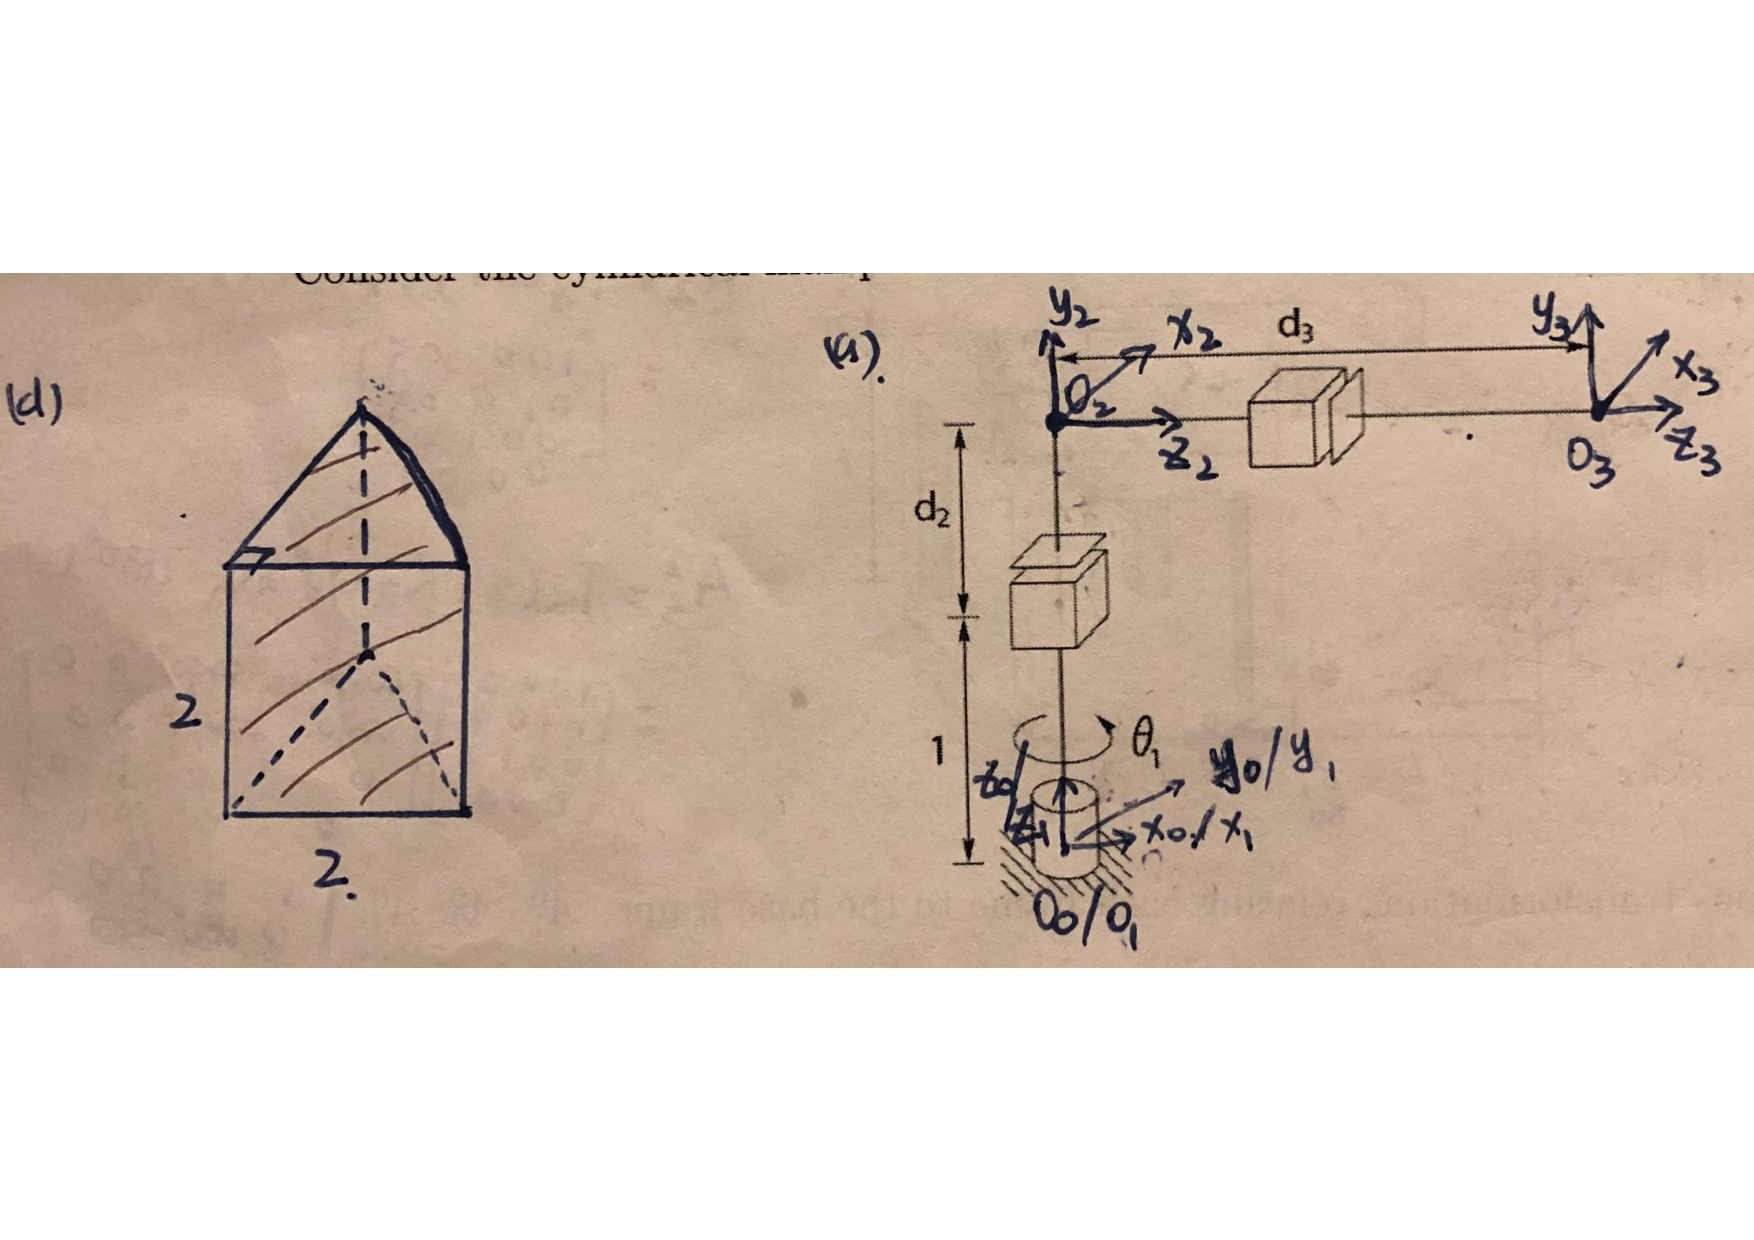
\includegraphics[scale=0.55]{p3}
%\caption{Coordinate frames on the manipulator.}
%\label{F2}
%\end{figure}
%%%%%%%%%%%%%%%%%%%%%%%%%%%%%%%%%%%%%%%%%%%%%%%%%%%%%%
%%
%\\\\
(b)\\
%
%%%%%%%%%%%%%%%%%%% Table. 2 %%%%%%%%%%%%%%%%%%%%%%%%%%%%%%
\begin{table}[h!] \centering
\caption{DH Parameter Table}
\begin{tabular}{|l|l|l|l|l|}
\hline
Link & $a_i$ & \textbf{$\alpha_i$} & $d_i$   & $\theta_i$ \\ \hline
1             & 0             & 0                 & 0      & $\theta_1$ \\ \hline
2             & 0             & 90                & $d_2+1$ & 90       \\ \hline
3             & 0             & 0                 & $d_3$   & 0        \\ \hline
\end{tabular}
\end{table}
%
\\\\
(c)
\begin{equation}
\begin{split}
A_1^0 &= R_z(\theta_1) = \left[
\begin{matrix}
\cos \theta_1 & -\sin \theta_1 & 0 & 0 \\
\sin \theta_1  & \cos \theta_1 & 0 & 0 \\
0 & 0 & 1 & 0 \\
0 & 0 & 0 & 1
\end{matrix}
\right]
\\
A_2^1 &= R_z(90)T_z(d_2+1)R_x(90) 
=
\begin{bmatrix}
0 & -1 & 0 & 0 \\
1 & 0 & 0& 0 \\
0 & 0 & 1 &0\\
0 & 0 & 0 & 1 
\end{bmatrix}
\begin{bmatrix}
1 & 0 & 0 & 0 \\
0 & 1 & 0& 0 \\
0 & 0 & 1 &d_2+1\\
0 & 0 & 0 & 1 
\end{bmatrix}
\begin{bmatrix}
1 & 0 & 0 & 0 \\
0 & 0 & -1 & 0 \\
0 & 1 & 0 & 0 \\
0 & 0 & 0 & 1 
\end{bmatrix}
\\
&=
\begin{bmatrix}
0 & 0 & -1 & 0 \\
-1 & 0 & 0 & 0 \\
0 & 1 & 0 & d_2+1 \\
0 & 0 & 0 & 1 
\end{bmatrix}
\\
A_3^2 &= T_z(d_3) = \begin{bmatrix}
1 & 0 & 0 & 0 \\
0 & 1 & 0& 0 \\
0 & 0 & 1 &d_3\\
0 & 0 & 0 & 1 
\end{bmatrix}
\end{split}
\end{equation}
So we have:
\begin{equation}
T_n^0 = A_1^0 A_2^1 A_3^2 = \left[
\begin{matrix}
\cos \theta_1 & -\sin \theta_1 & 0 & 0 \\
\sin \theta_1  & \cos \theta_1 & 0 & 0 \\
0 & 0 & 1 & 0 \\
0 & 0 & 0 & 1
\end{matrix}
\right]
\begin{bmatrix}
0 & 0 & -1 & 0 \\
-1 & 0 & 0 & 0 \\
0 & 1 & 0 & d_2+1 \\
0 & 0 & 0 & 1 
\end{bmatrix}
\begin{bmatrix}
1 & 0 & 0 & 0 \\
0 & 1 & 0& 0 \\
0 & 0 & 1 &d_3\\
0 & 0 & 0 & 1 
\end{bmatrix}
\end{equation}
\\\\
(d)
The workspace of the arm is 1/4 of a cylinder with radius = 2 and height = 2, shown in Fig. 2.

%%%%%%%%%%%%%%%%%%%%%%%%%%%%%%%%%%%%%%%%%%%%%%%%%%%%%
\section*{Problem 4}
(a)\\
Given only an arbitrary desired position of the end effector, there may be different number of solutions to the inverse kinematics problem.
If the desired position is inside the robot's workspace's boundary, there is infinite solutions;
if the desired position is on the boundary, there is only one solution;
if the desired position is outside the boundary, there is no solution.

If the orientation is also specified: 
if the desired position is inside the robot's workspace's boundary, there is one solution;
if the desired position is on the boundary, there may be 0 or 1 solution;
if the desired position is outside the boundary, there is no solution.
\\\\
(b)\\
Given $(p_x, p_y)$ and $\phi$, we want to solve the equations of $(\theta_1, d_2, \theta_3)$:
%
\begin{equation}
\begin{split}
p_x &= d_2 \cos \theta_1 + a_3 \cos(\theta_1 + \theta_3) \\
p_y &= d_2 \sin \theta_1 + a_3 \sin(\theta_1 + \theta_3) \\
\phi &= \theta_1 + \theta_3
\end{split}
\end{equation}
%
\begin{equation}
\begin{split}
p_x &= d_2 \cos \theta_1 + a_3 \cos \phi \\
p_y &= d_2 \sin \theta_1 + a_3 \sin \phi
\end{split}
\end{equation}
So we have the solution:
%
\begin{equation}
\begin{split}
d_2 &= \sqrt{(p_x - a_3 \cos \phi)^2 + (p_y - a_3 \sin\phi)^2}\\
\theta_1 &= Atan2 (p_y - a_3 \sin\phi, p_x - a_3 \cos \phi) \\
\theta_3 &= \phi - Atan2 (p_y - a_3 \sin\phi, p_x - a_3 \cos \phi)
\end{split}
\end{equation}
%

%%%%%%%%%%%%%%%%%%%%%%%%%%%%%%%%%%%%%%%%%%%%%%%%%%%%%
\section*{Problem 5}
(a)\\
%
%%%%%%%%%%%%%%%%%%% Table. 3 %%%%%%%%%%%%%%%%%%%%%%%%%%%%%%
\begin{table}[h!] \centering
\caption{DH Parameter Table}
\begin{tabular}{|l|l|l|l|l|}
\hline
Link & $a_i$ & $\alpha_i$ & $d_i$ & $\theta_i$ \\ \hline
1             & 0             & -90               & 0    & $\theta_1$    \\ \hline
2             & 0             & 90                & 0    & $\theta_2$    \\ \hline
3             & 45            & -90               & 550  & $\theta_3$    \\ \hline
4             & -45           & 90                & 0    & $\theta_4$    \\ \hline
5             & 0             & -90               & 300  & $\theta_5$    \\ \hline
6             & 0             & 90                & 0    & $\theta_6$    \\ \hline
7             & 0             & 0                 & 60   & $\theta_7$    \\ \hline
\end{tabular}
\end{table}
\\\\
(b)\\
In the Problem5.py, the program that implements the forward kinematics of the WAM arm is provided.
The function DHtransform takes input as (a, alpha, d, theta) and outputs the corresponding transform matrix.
The function WAM implements the WAH arm, which is composed of seven rotation joints with DH table from part (a).
One input parameter ltheta is $(\theta_1, \cdots, \theta_7)$ in the DH table, which is read from the qdata.txt. 
WAM performs transformation of the input matrix xe and output the matrix in the base frame. 
If we take xe as an indentity matrix with rank 4 , its [0, 3], [1,3] and [2,3] elements are the 3-D position in the base frame $O_0$.
Then we record every 3-D position of every movement, which is the trajectory of the marker tip.
The trajectory is shown in Fig. 3, 3 letters of 'kdc'.
%%
%%%%%%%%%%%%%%%%%%%% Fig. 1 %%%%%%%%%%%%%0%%%%%%%%%%%%%%%%%
%\begin{figure}[h!]
%\centering
%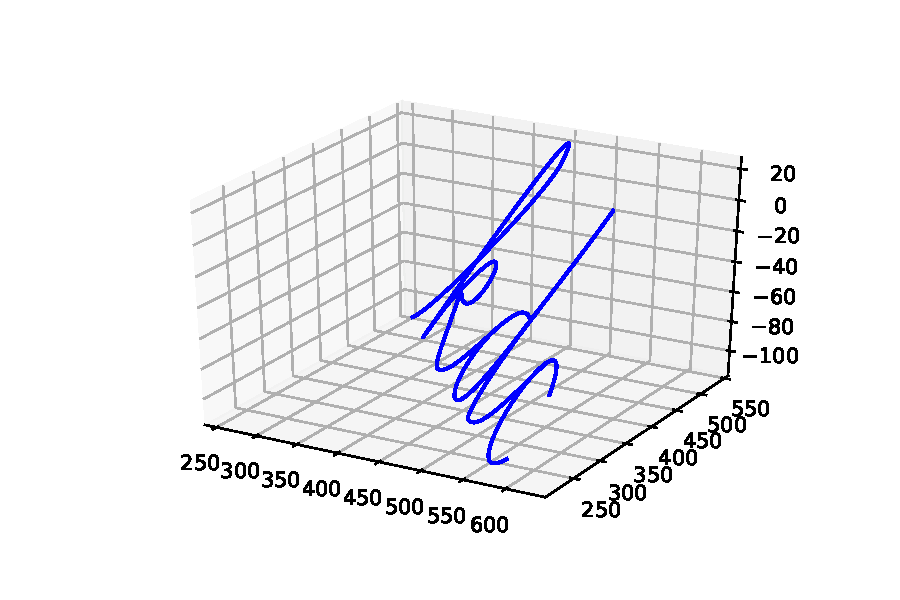
\includegraphics[scale=1]{p5}
%\caption{The trajectory of the marker tip with respect to the base frame $O_0$ and the sketch of the workspace.}
%\label{F3}
%\end{figure}
%%%%%%%%%%%%%%%%%%%%%%%%%%%%%%%%%%%%%%%%%%%%%%%%%%%%%%
%%
\end{document}
